%-------------------------------------------------------------------------------
% Figure of the proposed architecture
\begin{figure}[]
     \centering
     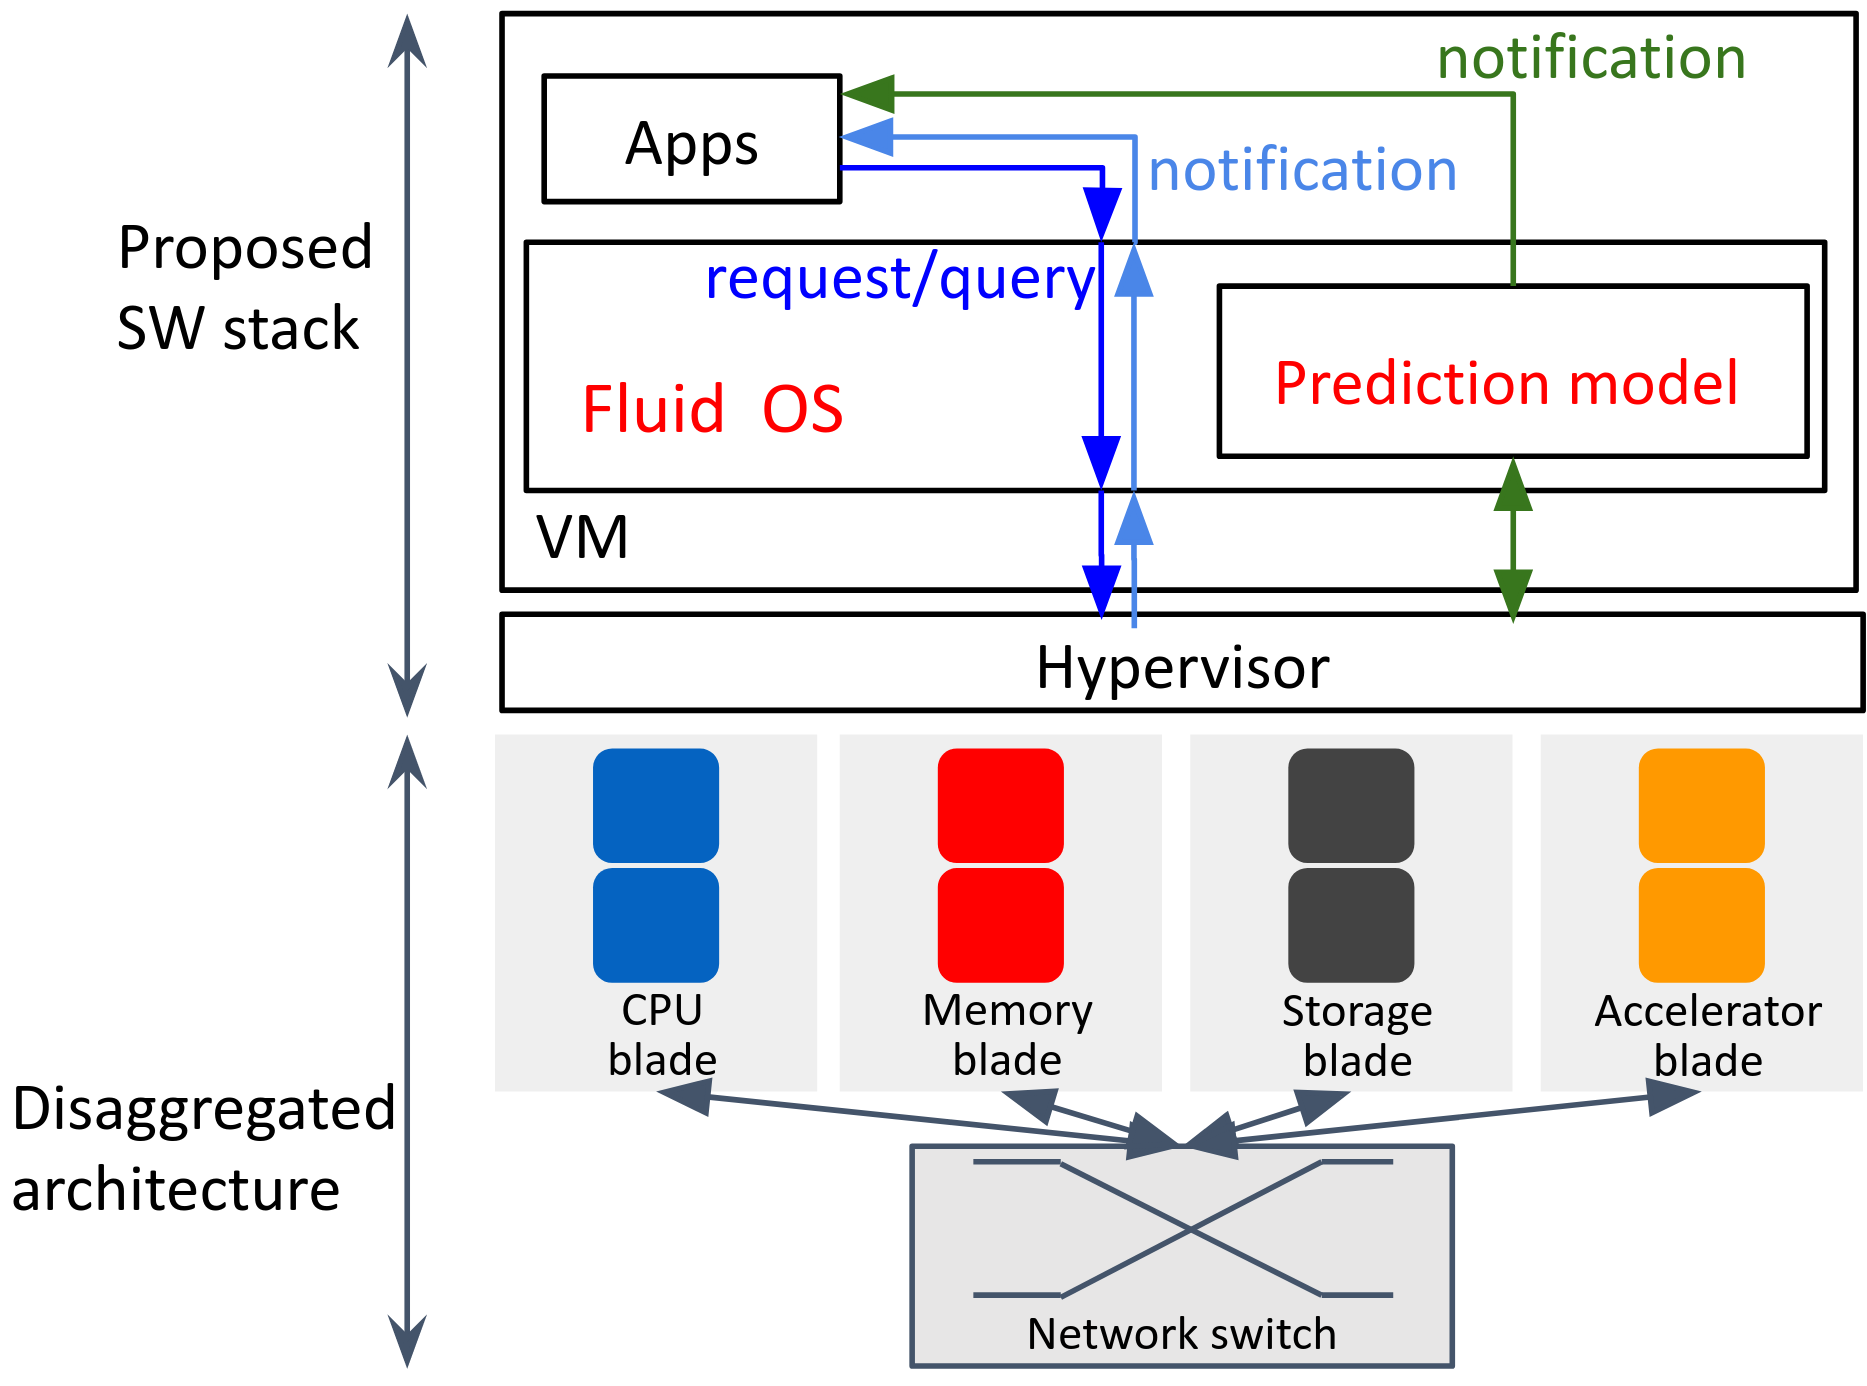
\includegraphics[scale=0.15]{images/architecture.png}
     \caption{Proposed architecture.}
     \label{fig:archi}
\end{figure}
%-------------------------------------------------------------------------------

\subsection{Previous works} \cite{sedaghat2013virtual} describes various VM
repacking policies that take either changes in workload or the total load as
input and output a decision on whether to reconfigure, and if so, the new
optimal resource distribution.  For memory-intensive workloads, a study of cloud
providers shows that auto-scaling of the memory resources can be accomplished by
analyzing the applications' memory miss ratio curve (MRC) and modeling it as a
hyperbola~\cite{novak2020auto}.

Prior research on web applications~\cite{yazdanov2014lightweight} shows that
fine-grained vertical scaling of multi-tiered web applications can be
accomplished through online reinforcement learning models.  Additionally, with
the recent development of machine learning models, prediction of the optimal
amount of resources can also be attained by certain supervised deep learning
models.  Since the input is a series of time-correlated data, recurrent neural
networks can capture the important features~\cite{gers1999learning}.

\cite{farokhi2016hybrid} suggests to use a control-theoretic approach to decide
how to vertical scale resources in web-facing applications.  They propose a
hybrid between two specific approaches: the performance-based (PC) approach and
capacity-based (CC) approach.  PC directly optimizes application performance
while CC focuses on optimizing resource utilization.  The paper shows that
combining these two approaches can combine the benefits.

\subsection{Our proposed approach} We tend to use neural nets with careful
design to support online learning. Before constructing a machine learning model,
it is essential to develop a clear understanding of what data to collect.
Similar to the heuristic method~\cite{sedaghat2013virtual}, a model accepts
traces of workload performance (e.g., latency, quality of services) and the
original VM configurations (e.g., number of CPU cores, memory size, and storage
size) as input and determines the best resource distribute for the workload.
For data collection, there exist powerful tools for monitoring performance, like
Prometheus~\cite{sukhija2019towards} and Grafana~\cite{Grafana}, which introduce
low overhead on fetching raw training data.  It may be beneficial to have
separate models for learning the best allocation for different types of
resources, for instance, one model focusing on the optimal number of cores, and
another model focusing on the optimal memory size.

Since reallocation of resources introduces overhead, the frequency of
reconfiguration must be constrained.  Analysis of such overheads may determine
selection between using a heuristic method or machine learning.  To minimize the
runtime overhead of machine learning, the models could be trained offline with
the collected data~\cite{zhang2019learned}. Deep learning models need a lot of
data, and therefore the space overhead is also a significant consideration.
